\documentclass[border=5mm]{standalone}
\usepackage[european]{circuitikz}
\usepackage[T1]{fontenc}\usepackage{helvet}\renewcommand{\familydefault}{\sfdefault}
\usetikzlibrary{arrows.meta,shadings,patterns,decorations.pathmorphing,calc,shadows.blur,spy}
\definecolor{stahl}{HTML}{C9CED6}\definecolor{stahlh}{HTML}{E7EAEE}\definecolor{stahld}{HTML}{8A929E}
\definecolor{heiss}{HTML}{E4572E}\definecolor{folie}{HTML}{BFD7EA}\definecolor{ware}{HTML}{F1DDB0}
\definecolor{band}{HTML}{33373D}\definecolor{dunkel}{HTML}{1F3A5F}\definecolor{ral}{HTML}{D7DBE0}
\tikzset{
 k/.style={line width=0.8pt,draw=black,line join=round},
 nr/.style={circle,draw=black,fill=white,line width=0.7pt,inner sep=1pt,font=\bfseries\footnotesize,minimum size=5mm},
 hl/.style={line width=0.45pt,-{Circle[length=2pt]}},
 schraube/.style={fill=stahld,draw=black,line width=0.3pt},
}
% Schrägbild: Tiefe
\def\dx{0.45}\def\dy{0.3}
% Quader: x y Breite Höhe Tiefe Farbe
\newcommand{\quader}[6]{%
 \fill[#6!75!black,draw=black,line width=0.8pt,line join=round] (#1+#3,#2) -- ++(#5*\dx,#5*\dy) -- ++(0,#4) -- ++(-#5*\dx,-#5*\dy) -- cycle;
 \fill[#6!45!white,draw=black,line width=0.8pt,line join=round] (#1,#2+#4) -- ++(#5*\dx,#5*\dy) -- ++(#3,0) -- ++(-#5*\dx,-#5*\dy) -- cycle;
 \shade[top color=#6!85!white,bottom color=#6,draw=black,line width=0.8pt] (#1,#2) rectangle ++(#3,#4);
 \draw[k] (#1,#2) rectangle ++(#3,#4);}
\newcommand{\schale}[3]{% x, Folie(0/1), Farbe der Folie
 \fill[black!15,blur shadow={shadow blur steps=5,shadow xshift=0.5pt,shadow yshift=-0.5pt}] (#1+0.1,2.36) ellipse (0pt and 0pt);
 \draw[k,fill=white] (#1,2.28) -- ++(0.12,0.5) -- ++(1.1,0) -- ++(0.12,-0.5) -- cycle;
 \draw[k,fill=white!92!black] (#1+0.12,2.78) -- ++(\dx*0.9,\dy*0.9) -- ++(1.1,0) -- ++(-\dx*0.9,-\dy*0.9) -- cycle;
 \fill[ware] (#1+0.22,2.38) rectangle ++(0.9,0.3);
 \fill[ware!80!brown] (#1+0.22+0.1,2.78+0.04) -- ++(\dx*0.6,\dy*0.6) -- ++(0.7,0) -- ++(-\dx*0.6,-\dy*0.6) -- cycle;
 \ifnum#2=1 \fill[#3,opacity=0.75,draw=dunkel,line width=0.6pt] (#1+0.08,2.8) -- ++(\dx*0.95,\dy*0.95) -- ++(1.18,0) -- ++(-\dx*0.95,-\dy*0.95) -- cycle;\fi}
\begin{document}
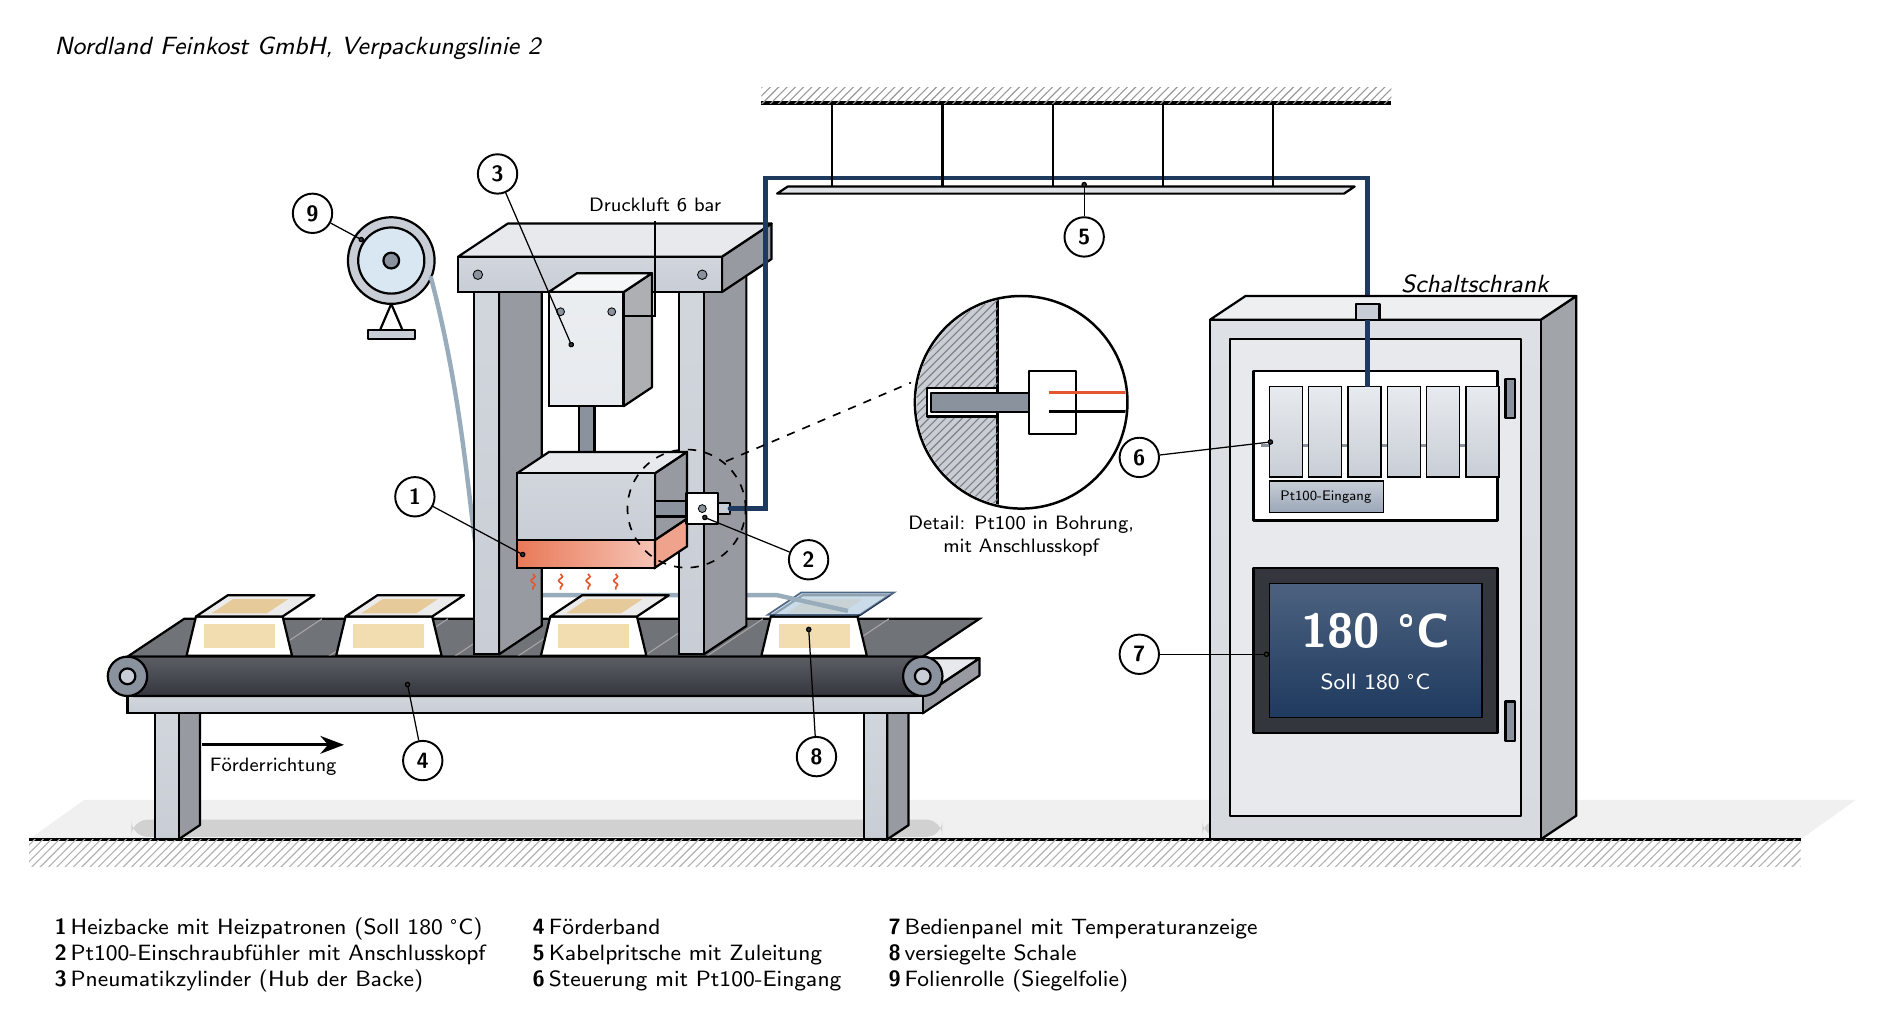
\begin{tikzpicture}[x=1cm,y=1cm]
%================ Boden mit Schatten
\fill[black!6] (-1,-0.05) -- (21.5,-0.05) -- (22.2,0.45) -- (-0.3,0.45) -- cycle;
\draw[line width=1pt] (-1,-0.05) -- (21.5,-0.05);
\fill[pattern=north east lines,pattern color=black!30] (-1,-0.4) rectangle (21.5,-0.05);
\foreach \x/\w in {0.3/10.3,13.9/4.3}{\fill[black!18,rounded corners=6pt] (\x,-0.02) rectangle ++(\w,0.22);}
%================ Gestell
\foreach \x in {0.6,9.6}{\quader{\x}{-0.05}{0.3}{1.65}{0.6}{stahl}}
\quader{0.25}{1.55}{10.1}{0.22}{1.6}{stahl}
%================ Förderband (Schrägbild)
\fill[band!70!white,draw=black,line width=0.8pt] (0.25,2.27) -- ++(1.6*\dx,1.6*\dy) -- ++(10.1,0) -- ++(-1.6*\dx,-1.6*\dy) -- cycle;
\foreach \x in {1.2,2.0,...,9.6}{\draw[white!55!band,line width=0.4pt] (\x,2.27) -- ++(1.6*\dx,1.6*\dy);}
\shade[top color=band!80!white,bottom color=band,draw=black,line width=0.8pt,rounded corners=2pt] (0.25,1.77) rectangle (10.35,2.27);
\foreach \x in {0.25,10.35}{\draw[k,fill=stahld] (\x,2.02) circle (0.25); \draw[k,fill=stahl] (\x,2.02) circle (0.1);}
\draw[-{Stealth[length=3mm]},line width=1pt] (1.2,1.15)--(3.0,1.15) node[midway,below=1pt,font=\scriptsize]{Förderrichtung};
%================ Schalen
\schale{1.0}{0}{folie}\schale{2.9}{0}{folie}\schale{8.3}{1}{folie}
%================ Folienrolle und Folienbahn
\draw[k,fill=stahl] (3.6,7.3) circle (0.55); \draw[k,fill=folie!60!white] (3.6,7.3) circle (0.42); \draw[k,fill=stahld] (3.6,7.3) circle (0.1);
\draw[k] (3.6,6.75) -- (3.45,6.4) (3.6,6.75) -- (3.75,6.4); \draw[k,fill=stahl] (3.3,6.3) rectangle (3.9,6.42);
\draw[folie!80!black,line width=1.6pt] (4.1,7.1) .. controls (4.6,5.2) and (4.6,3.6) .. (4.8,3.05) -- (8.5,3.05) -- (9.4,2.85);
%================ Portal der Siegelstation
\quader{4.65}{2.3}{0.32}{4.6}{1.2}{stahl}
\quader{7.25}{2.3}{0.32}{4.6}{1.2}{stahl}
\quader{4.45}{6.9}{3.35}{0.45}{1.4}{stahl}
\foreach \x in {4.7,7.55}{\fill[schraube] (\x,7.12) circle (0.06);}
% Pneumatikzylinder
\quader{5.6}{5.45}{0.95}{1.45}{0.8}{stahlh}
\draw[k,fill=stahld] (5.98,4.6) rectangle (6.18,5.45);
\fill[schraube] (5.75,6.65) circle (0.05); \fill[schraube] (6.4,6.65) circle (0.05);
\draw[line width=0.7pt] (6.55,6.6) -- (6.95,6.6) -- (6.95,7.8) node[above,font=\scriptsize]{Druckluft 6 bar};
% Heizbacke mit Heizpatrone und Pt100-Bohrung
\quader{5.2}{3.75}{1.75}{0.85}{0.9}{stahl}
\shade[left color=heiss!80,right color=heiss!35,draw=black,line width=0.8pt] (5.2,3.4) rectangle (6.95,3.75);
\fill[heiss!55,draw=black,line width=0.8pt] (6.95,3.4) -- ++(0.9*\dx,0.9*\dy) -- ++(0,0.35) -- ++(-0.9*\dx,-0.9*\dy) -- cycle;
\foreach \x in {5.4,5.75,...,6.8}{\draw[heiss,line width=0.6pt,decorate,decoration={snake,amplitude=0.7pt,segment length=3pt}] (\x,3.32)--(\x,3.12);}
\schale{5.5}{0}{folie}
% Pt100-Fühler (Einschraubfühler) mit Anschlusskopf
\draw[k,fill=stahld] (6.95,4.05) rectangle (7.35,4.25);
\draw[k,fill=white] (7.35,3.95) rectangle (7.75,4.35); \fill[schraube] (7.55,4.15) circle (0.05);
\draw[k,fill=stahl] (7.75,4.08) rectangle (7.9,4.22);
%================ Zuleitung in Kabelpritsche
\draw[dunkel,line width=1.6pt,line cap=round] (7.9,4.15) -- (8.35,4.15) -- (8.35,8.35) -- (16.0,8.35) -- (16.0,6.6);
\draw[k,fill=stahl!60] (8.5,8.15) -- ++(0.3*\dx,0.3*\dy) -- ++(7.2,0) -- ++(-0.3*\dx,-0.3*\dy) -- cycle;
\foreach \x in {9.2,10.6,...,15.2}{\draw[k,fill=stahld] (\x,8.25) -- (\x,9.3);}
\draw[line width=1.2pt] (8.3,9.3) -- (16.3,9.3);
\fill[pattern=north east lines,pattern color=black!40] (8.3,9.3) rectangle (16.3,9.5);
%================ Schaltschrank (Schrägbild)
\quader{14.0}{-0.05}{4.2}{6.6}{1.0}{ral}
\draw[k,fill=ral!60!white] (14.25,0.25) rectangle (17.95,6.3);
\foreach \y in {1.2,5.3}{\draw[k,fill=stahld] (17.75,\y) rectangle ++(0.12,0.5);}
\draw[k,fill=stahl] (15.85,6.55) -- ++(0.3,0) -- ++(0,0.2) -- ++(-0.3,0) -- cycle;
% Steuerung auf Hutschiene
\draw[k,fill=white] (14.55,4.0) rectangle (17.65,5.9);
\draw[line width=1pt,stahld] (14.65,4.95) -- (17.55,4.95);
\foreach \x in {14.75,15.25,...,17.3}{\shade[top color=stahlh,bottom color=stahl,draw=black,line width=0.5pt] (\x,4.55) rectangle ++(0.42,1.15);}
\shade[top color=dunkel!25,bottom color=dunkel!45,draw=black,line width=0.5pt] (14.75,4.1) rectangle (16.2,4.5);
\node[font=\tiny] at (15.47,4.3) {Pt100-Eingang};
\draw[dunkel,line width=1.6pt] (16.0,6.55) -- (16.0,5.7);
% Bedienpanel
\draw[k,fill=band] (14.55,1.3) rectangle (17.65,3.4);
\shade[top color=dunkel!80,bottom color=dunkel,draw=black,line width=0.5pt] (14.75,1.5) rectangle (17.45,3.2);
\node[white,font=\bfseries\LARGE] at (16.1,2.6) {180 °C};
\node[white,font=\footnotesize] at (16.1,1.95) {Soll 180 °C};
%================ Detail-Lupe Pt100
\draw[line width=0.6pt,dashed] (7.35,4.15) circle (0.75);
\draw[line width=0.6pt,dashed] (7.85,4.75) -- (10.2,5.75);
\begin{scope}[shift={(11.6,5.5)}]
 \fill[white,draw=black,line width=0.9pt] (0,0) circle (1.35);
 \begin{scope}
 \clip (0,0) circle (1.33);
 \fill[stahl] (-1.4,-1.4) rectangle (-0.3,1.4); \draw[k] (-0.3,-1.4)--(-0.3,1.4);
 \fill[pattern=north east lines,pattern color=black!50] (-1.4,-1.4) rectangle (-0.3,1.4);
 \fill[white] (-1.2,-0.18) rectangle (-0.3,0.18); \draw[k] (-1.2,-0.18) rectangle (-0.3,0.18);
 \draw[k,fill=stahld] (-1.15,-0.12) rectangle (0.1,0.12);
 \draw[k,fill=white] (0.1,-0.4) rectangle (0.7,0.4);
 \draw[line width=1pt,heiss] (0.35,0.12) -- (1.4,0.12);
 \draw[line width=1pt,black] (0.35,-0.12) -- (1.4,-0.12);
 \end{scope}
 \node[font=\scriptsize,align=center] at (0,-1.7) {Detail: Pt100 in Bohrung,\\mit Anschlusskopf};
\end{scope}
%================ Positionsnummern
\node[nr] (n1) at (3.9,4.3) {1}; \draw[hl] (n1) -- (5.3,3.55);
\node[nr] (n2) at (8.9,3.5) {2}; \draw[hl] (n2) -- (7.55,4.05);
\node[nr] (n3) at (4.95,8.4) {3}; \draw[hl] (n3) -- (5.9,6.2);
\node[nr] (n4) at (4.0,0.95) {4}; \draw[hl] (n4) -- (3.8,1.95);
\node[nr] (n5) at (12.4,7.6) {5}; \draw[hl] (n5) -- (12.4,8.3);
\node[nr] (n6) at (13.1,4.8) {6}; \draw[hl] (n6) -- (14.8,5.0);
\node[nr] (n7) at (13.1,2.3) {7}; \draw[hl] (n7) -- (14.75,2.3);
\node[nr] (n8) at (9.0,1.0) {8}; \draw[hl] (n8) -- (8.9,2.65);
\node[nr] (n9) at (2.6,7.9) {9}; \draw[hl] (n9) -- (3.25,7.55);
%================ Beschriftung Bereiche
\node[font=\small\itshape,anchor=west] at (-0.8,10.0) {Nordland Feinkost GmbH, Verpackungslinie 2};
\node[font=\small\itshape,anchor=west] at (16.3,7.0) {Schaltschrank};
%================ Legende
\begin{scope}[shift={(-0.8,-0.9)}]
\node[anchor=north west,font=\footnotesize,align=left] at (0,0){%
\begin{tabular}{@{}r@{\,}l@{\qquad}r@{\,}l@{\qquad}r@{\,}l@{}}
\textbf{1} & Heizbacke mit Heizpatronen (Soll 180 °C) & \textbf{4} & Förderband & \textbf{7} & Bedienpanel mit Temperaturanzeige\\
\textbf{2} & Pt100-Einschraubfühler mit Anschlusskopf & \textbf{5} & Kabelpritsche mit Zuleitung & \textbf{8} & versiegelte Schale\\
\textbf{3} & Pneumatikzylinder (Hub der Backe) & \textbf{6} & Steuerung mit Pt100-Eingang & \textbf{9} & Folienrolle (Siegelfolie)
\end{tabular}};
\end{scope}
\end{tikzpicture}
\end{document}
